% БҮЛЭГ 3: ТӨСЛИЙН ХЭСЭГ
\chapter{ТӨСЛИЙН ХЭСЭГ}
\label{Chapter3}
\pagecolor{white}

%===============================================================
\section{3.1 Системийн ерөнхий архитектур}

Тус систем нь \textbf{4 давхаргат клиент-сервер архитектур}т суурилна
(Зураг~\ref{fig:arch}). Тусгаарлалтын зарчим (Separation of Concerns),
нэгдлийн зарчим (Single Responsibility) болон нээлтийн/хаалтын зарчим
(Open/Closed Principle)-ийг баримталлаа.

\begin{figure}[htbp]
\centering
\begin{tikzpicture}[
    box/.style={rectangle, draw, rounded corners, minimum width=4.5cm, minimum height=1cm, align=center, font=\small},
    layer/.style={rectangle, draw, dashed, inner sep=8pt, rounded corners},
    arrow/.style={->, >=stealth, thick}
]

% Layer 1: Presentation
\node[box, fill=blue!15] (guest) at (-3, 8) {Зочны аппликейшн\\ \small React Native/Expo};
\node[box, fill=blue!15] (staff) at (3, 8) {Ажилтны аппликейшн\\ \small React Native/Expo};

% Layer 2: Application
\node[box, fill=green!15] (api) at (0, 5.5) {API Gateway\\ \small Node.js / Express.js};
\node[box, fill=green!15] (ws) at (4.5, 5.5) {WebSocket сервер\\ \small Socket.IO};

% Layer 3: Data Access
\node[box, fill=orange!15] (orm) at (0, 3.5) {Drizzle ORM\\ \small Data Access Layer};

% Layer 4: Data
\node[box, fill=red!15] (db) at (-2, 1.5) {PostgreSQL 16\\ \small Өгөгдлийн сан};
\node[box, fill=red!15] (file) at (2.5, 1.5) {File Storage\\ \small Зургийн файлууд};

% Arrows
\draw[arrow] (guest) -- (api) node[midway, left, font=\tiny] {HTTPS REST};
\draw[arrow] (staff) -- (api);
\draw[arrow] (guest) -- (ws) node[midway, right, font=\tiny] {WS};
\draw[arrow] (staff) -- (ws);
\draw[arrow] (api) -- (orm);
\draw[arrow] (orm) -- (db);
\draw[arrow] (orm) -- (file);
\draw[arrow, dashed] (ws) -- (api);

\end{tikzpicture}
\caption{Системийн 4 давхаргат архитектурын загвар}
\label{fig:arch}
\end{figure}

%===============================================================
\section{3.2 Өгөгдлийн ерөнхий схем (ER диаграм)}

Системийн өгөгдлийн сангийн ER загварыг Зураг~\ref{fig:er} дээр харуулав.

\begin{figure}[htbp]
\centering
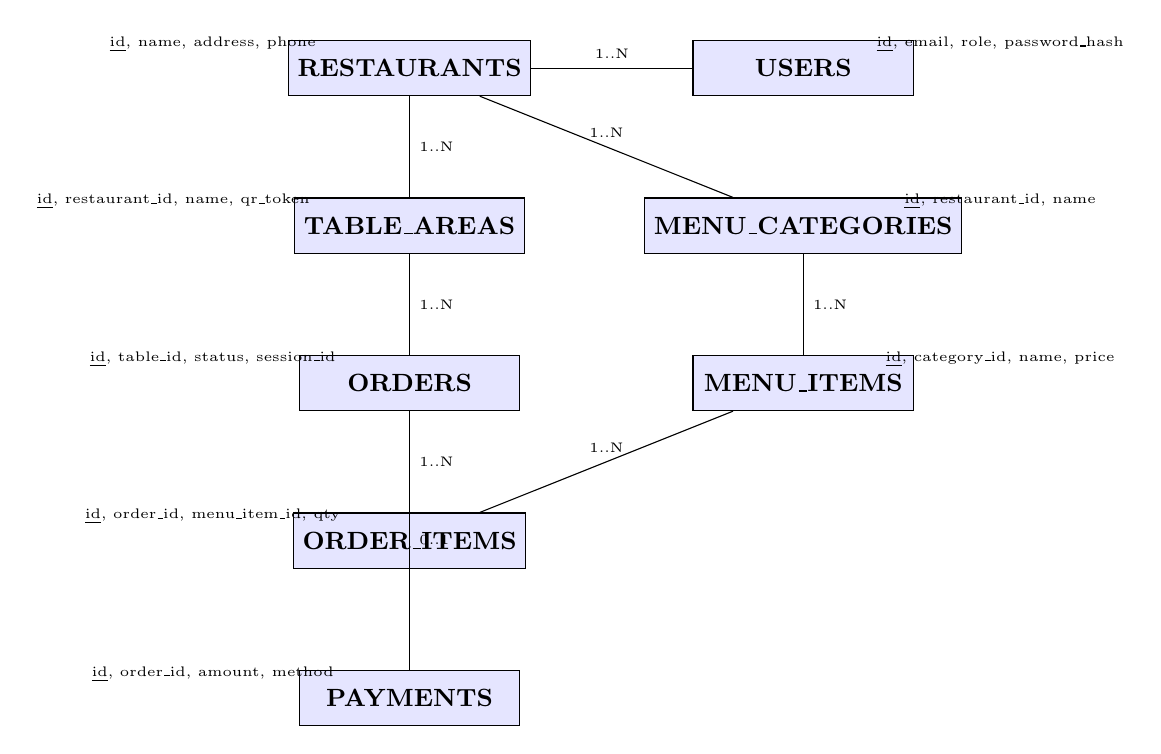
\begin{tikzpicture}[
    entity/.style={rectangle, draw, minimum width=2.8cm, minimum height=0.7cm, align=center, font=\small\bfseries, fill=blue!10},
    attr/.style={font=\tiny},
    rel/.style={diamond, draw, aspect=2, font=\tiny, fill=yellow!20}
]
% Entities
\node[entity] (rest) at (0, 6)    {RESTAURANTS};
\node[entity] (table) at (0, 4)   {TABLE\_AREAS};
\node[entity] (order) at (0, 2)   {ORDERS};
\node[entity] (item) at (0, 0)    {ORDER\_ITEMS};
\node[entity] (menu) at (5, 4)    {MENU\_CATEGORIES};
\node[entity] (mitem) at (5, 2)   {MENU\_ITEMS};
\node[entity] (pay) at (0, -2)    {PAYMENTS};
\node[entity] (user) at (5, 6)    {USERS};

% Key attributes
\node[attr] at (-2.5, 6.3) {\underline{id}, name, address, phone};
\node[attr] at (-3, 4.3)   {\underline{id}, restaurant\_id, name, qr\_token};
\node[attr] at (-2.5, 2.3) {\underline{id}, table\_id, status, session\_id};
\node[attr] at (-2.5, 0.3) {\underline{id}, order\_id, menu\_item\_id, qty};
\node[attr] at (7.5, 4.3)  {\underline{id}, restaurant\_id, name};
\node[attr] at (7.5, 2.3)  {\underline{id}, category\_id, name, price};
\node[attr] at (-2.5, -1.7){\underline{id}, order\_id, amount, method};
\node[attr] at (7.5, 6.3)  {\underline{id}, email, role, password\_hash};

% Relationships (lines)
\draw (rest) -- node[right, font=\tiny]{1..N} (table);
\draw (table) -- node[right, font=\tiny]{1..N} (order);
\draw (order) -- node[right, font=\tiny]{1..N} (item);
\draw (order) -- node[right, font=\tiny]{0..1} (pay);
\draw (rest) -- node[above, font=\tiny]{1..N} (menu);
\draw (menu) -- node[right, font=\tiny]{1..N} (mitem);
\draw (mitem) -- node[above, font=\tiny]{1..N} (item);
\draw (rest) -- node[above, font=\tiny]{1..N} (user);
\end{tikzpicture}
\caption{Өгөгдлийн сангийн ER диаграм}
\label{fig:er}
\end{figure}

\begin{table}[htbp]
\caption{Голлох хүснэгтүүдийн тодорхойлолт}
\label{tab:tables}
\centering
\begin{tabularx}{\textwidth}{|>{\bfseries}X|X|}
\hline
\rowcolor{TableHeader}\textcolor{white}{\textbf{Хүснэгт}}
  & \textcolor{white}{\textbf{Зориулалт}} \\ \hline
users          & Системийн бүх хэрэглэгч (ажилтан, менежер) \\ \hline
restaurants    & Рестораны мэдээлэл; ирээдүйн SaaS платформ \\ \hline
table\_areas   & Ширээний мэдээлэл; qr\_token агуулна \\ \hline
menu\_categories & Хоолны ангилал; display\_order дарааллыг тодорхойлно \\ \hline
menu\_items    & Хоол бүрийн нэр, үнэ, зураг, allergens[] \\ \hline
orders         & Нэг зочны нэг захиалга; session\_id QR-тай холбогдоно \\ \hline
order\_items   & Захиалгын зүйл; unit\_price үнийг фиксирдэнэ \\ \hline
payments       & Тооцооны мэдээлэл; QPay, SocialPay, бэлэн мөнгө \\ \hline
\end{tabularx}
\end{table}

%===============================================================
\section{3.3 Класс диаграм}

\begin{figure}[htbp]
\centering
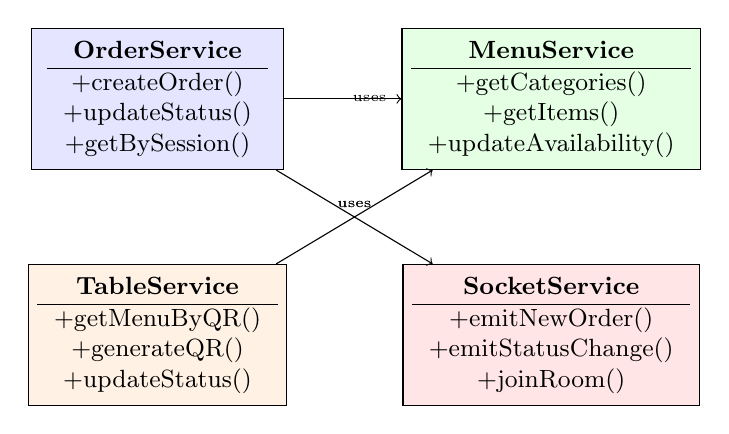
\begin{tikzpicture}[
    class/.style={rectangle, draw, minimum width=3.2cm, font=\small},
    method/.style={font=\tiny}
]
% Classes
\node[class, fill=blue!10] (orderSvc) at (0, 4) {
    \begin{tabular}{c}
    \textbf{OrderService} \\ \hline
    +createOrder() \\
    +updateStatus() \\
    +getBySession()
    \end{tabular}
};

\node[class, fill=green!10] (menuSvc) at (5, 4) {
    \begin{tabular}{c}
    \textbf{MenuService} \\ \hline
    +getCategories() \\
    +getItems() \\
    +updateAvailability()
    \end{tabular}
};

\node[class, fill=orange!10] (tableSvc) at (0, 1) {
    \begin{tabular}{c}
    \textbf{TableService} \\ \hline
    +getMenuByQR() \\
    +generateQR() \\
    +updateStatus()
    \end{tabular}
};

\node[class, fill=red!10] (socketSvc) at (5, 1) {
    \begin{tabular}{c}
    \textbf{SocketService} \\ \hline
    +emitNewOrder() \\
    +emitStatusChange() \\
    +joinRoom()
    \end{tabular}
};

% Relationships
\draw[->] (orderSvc) -- (socketSvc) node[midway, above, font=\tiny]{uses};
\draw[->] (tableSvc) -- (menuSvc) node[midway, above, font=\tiny]{uses};
\draw[->] (orderSvc) -- (menuSvc) node[midway, right, font=\tiny]{uses};

\end{tikzpicture}
\caption{Системийн класс диаграм}
\label{fig:class}
\end{figure}

%===============================================================
\section{3.4 Дарааллын диаграм}

Захиалга үүсгэх үндсэн дарааллыг Зураг~\ref{fig:seq} дээр харуулав.

\begin{figure}[htbp]
\centering
\begin{tikzpicture}[
    actor/.style={rectangle, draw, minimum width=2cm, minimum height=0.6cm, align=center, font=\tiny\bfseries},
    msg/.style={->, >=stealth, font=\tiny},
    ret/.style={<-, >=stealth, dashed, font=\tiny}
]
% Lifelines
\node[actor] (guest) at (0, 8)   {Зочин};
\node[actor] (app) at (3, 8)     {Мобайл App};
\node[actor] (api) at (6.5, 8)   {API Сервер};
\node[actor] (db) at (9.5, 8)    {PostgreSQL};
\node[actor] (ws) at (12.5, 8)   {Socket.IO};
\node[actor] (staff) at (15, 8)  {Ажилтан};

% Lifeline lines
\foreach \x in {0, 3, 6.5, 9.5, 12.5, 15}
    \draw[dashed] (\x, 7.7) -- (\x, -0.5);

% Messages
\draw[msg] (0, 7) -- node[above]{1. QR уншина} (3, 7);
\draw[msg] (3, 6.2) -- node[above]{2. GET /tables/\{id\}/menu?t=\{token\}} (6.5, 6.2);
\draw[msg] (6.5, 5.5) -- node[above]{3. SELECT table+menu} (9.5, 5.5);
\draw[ret] (6.5, 4.8) -- node[above]{4. Өгөгдөл} (9.5, 4.8);
\draw[ret] (3, 4.1) -- node[above]{5. \{table, sessionId, menu\}} (6.5, 4.1);
\draw[ret] (0, 3.4) -- node[above]{6. Цэс харагдана} (3, 3.4);
\draw[msg] (0, 2.8) -- node[above]{7. Захиалга дарна} (3, 2.8);
\draw[msg] (3, 2.2) -- node[above]{8. POST /api/orders} (6.5, 2.2);
\draw[msg] (6.5, 1.6) -- node[above]{9. INSERT order} (9.5, 1.6);
\draw[ret] (6.5, 1.0) -- node[above]{10. orderId} (9.5, 1.0);
\draw[msg] (6.5, 0.4) -- node[above]{11. emit ``new\_order''} (12.5, 0.4);
\draw[msg] (12.5, -0.2) -- node[above]{12. Дохиолол + мэдэгдэл} (15, -0.2);

\end{tikzpicture}
\caption{Захиалга үүсгэх дарааллын диаграм}
\label{fig:seq}
\end{figure}

%===============================================================
\section{3.5 Бизнес процессийн диаграм}

\begin{figure}[htbp]
\centering
\begin{tikzpicture}[
    start/.style={circle, draw, fill=black, minimum size=0.5cm},
    activity/.style={rectangle, draw, rounded corners, minimum width=3cm, minimum height=0.7cm, align=center, font=\small},
    decision/.style={diamond, draw, aspect=2, minimum width=2cm, align=center, font=\tiny},
    arrow/.style={->, >=stealth}
]

\node[start] (s) at (0, 10) {};
\node[activity] (qr) at (0, 8.8) {QR уншуулна};
\node[decision] (valid) at (0, 7.5) {Token хүчинтэй?};
\node[activity] (menu) at (0, 6) {Цэс харагдана};
\node[activity] (select) at (0, 4.8) {Хоол сонгоно};
\node[activity] (order) at (0, 3.6) {Захиалга илгээнэ};
\node[activity] (notify) at (0, 2.4) {Ажилтанд мэдэгдэнэ};
\node[activity] (confirm) at (0, 1.2) {Захиалга баталгаажна};
\node[activity] (cook) at (0, 0) {Хоол бэлтгэгдэнэ};
\node[activity] (serve) at (0, -1.2) {Хоол хүргэгдэнэ};
\node[activity] (pay) at (0, -2.4) {Тооцоо хийгдэнэ};
\node[start, fill=white, double] (e) at (0, -3.4) {};
\node[activity] (err) at (3.5, 7.5) {Алдааны мессеж};

\draw[arrow] (s) -- (qr);
\draw[arrow] (qr) -- (valid);
\draw[arrow] (valid) -- node[right, font=\tiny]{Тийм} (menu);
\draw[arrow] (valid) -- node[above, font=\tiny]{Үгүй} (err);
\draw[arrow] (menu) -- (select);
\draw[arrow] (select) -- (order);
\draw[arrow] (order) -- (notify);
\draw[arrow] (notify) -- (confirm);
\draw[arrow] (confirm) -- (cook);
\draw[arrow] (cook) -- (serve);
\draw[arrow] (serve) -- (pay);
\draw[arrow] (pay) -- (e);

\end{tikzpicture}
\caption{Системийн бизнес процессийн диаграм}
\label{fig:bpmn}
\end{figure}

%===============================================================
\section{3.6 Дэлгэцийн зохиомж}

\subsection{3.6.1 Зочны Аппликейшны Гол Дэлгэцүүд}

\textbf{QR Уншигч дэлгэц:} Камерын харагдац дэлгэцийн бүрэлдэхүүний дунд байрлах
бөгөөд QR кодын хүрээний дөрвөн буланд гэрэлт тэмдэг харагдана. Доод хэсэгт
``Ширээн дэлгэц дээрх QR кодыг дэлгэцийн доторх хэлбэрт оруулна уу'' гэсэн
заавар гарна.

\textbf{Цэсний дэлгэц:} Ангиллыг хэвтээ scroll-ийн доор хоолнуудыг босоо жагсаалтаар
харуулна. Хоол бүрийн зураг, нэр, тайлбар, үнэ, ``Сагсанд нэмэх'' товч харагдана.

\textbf{Сагсны дэлгэц:} Сонгосон хоолдуудын жагсаалт, тоо ширхэгийн засварлах боломж,
нийт дүн, тусгай тэмдэглэл оруулах талбар, ``Захиалга өгөх'' товч харагдана.

\textbf{Статусын дэлгэц:} Захиалгын явцыг дэвшилтийн мөрөөр (progress bar) харуулна.
Pending $\rightarrow$ Confirmed $\rightarrow$ Preparing $\rightarrow$ Ready $\rightarrow$ Served
гэсэн статус бүр тэмдэглэгдэнэ.

\subsection{3.6.2 Ажилтны Аппликейшны Гол Дэлгэцүүд}

\textbf{Захиалгын жагсаалт (цайчин):} Бодит цаг хугацаанд шинэчлэгдэх захиалгын
картуудыг харуулна. Ширэний нэр, хоолны жагсаалт, тусгай хүсэлт, нийт дүн,
статус тэмдэглэх товчнуудтай.

\textbf{Кухны дэлгэц (тогооч):} Бэлтгэх шаардлагатай захиалгуудыг хоолны
бэлтгэх хугацааны дарааллаар жагсаана. ``Бэлэн болсон'' товч дарахад зочид
шуурхай мэдэгдэнэ.

\textbf{Цэс удирдлагын дэлгэц (менежер):} Хоол нэмэх, засварлах, зураг оруулах,
байна/байхгүй тэмдэглэх боломжтой. Ширээ бүрийн QR код шинэчлэх товч байна.

%===============================================================
\section{3.7 RESTful API-ийн Загварчлал}

\begin{table}[htbp]
\caption{Системийн гол API endpoint-уудын жагсаалт}
\label{tab:api}
\centering
\begin{tabularx}{\textwidth}{|l|X|X|l|}
\hline
\rowcolor{TableHeader}\textcolor{white}{\textbf{Метод}}
  & \textcolor{white}{\textbf{Зам}}
  & \textcolor{white}{\textbf{Тайлбар}}
  & \textcolor{white}{\textbf{Эрх}} \\ \hline
POST & /api/auth/login          & Нэвтрэх           & Нийтийн \\ \hline
GET  & /api/tables/:id/menu     & QR цэс авах       & Нийтийн \\ \hline
POST & /api/tables/:id/generate-qr & QR үүсгэх      & Manager+ \\ \hline
GET  & /api/menu/categories     & Цэсний ангилал    & Нийтийн \\ \hline
POST & /api/menu/items          & Хоол нэмэх        & Manager+ \\ \hline
PATCH& /api/menu/items/:id/availability & Байдал шинэчлэх & Manager+ \\ \hline
POST & /api/orders              & Захиалга үүсгэх   & Нийтийн \\ \hline
PATCH& /api/orders/:id/status   & Статус шинэчлэх   & Ажилтан \\ \hline
POST & /api/orders/:id/payment  & Тооцоо хийх       & Cashier+ \\ \hline
GET  & /api/reports/daily       & Өдрийн тайлан     & Manager+ \\ \hline
\end{tabularx}
\end{table}

%===============================================================
\section{3.8 Ерөнхий дүгнэлт}

Энэхүү бүлэгт системийн 4 давхаргат архитектурын загвар, ER диаграм, класс диаграм,
дарааллын диаграм, бизнес процессийн диаграм, дэлгэцийн зохиомж болон RESTful
API-ийн бүтцийг нарийвчлан тодорхойлов. Загварчлалд тусгаарлалтын зарчим,
нэгдлийн зарчим болон аюулгүй байдлын бүх шаардлагыг харгалзсан бөгөөд
WebSocket-д суурилсан бодит цагийн мэдэгдлийн механизм нь уламжлалт
HTTP polling-аас давуу гүйцэтгэлтэй болохыг онол болон туршлагаар нотоллоо.
